\documentclass[11pt]{article}
\usepackage[letterpaper,margin=1.0in,top=.86in,bottom=.88in]{geometry}
\usepackage[T1]{fontenc}
\usepackage{lmodern}
\usepackage{amsmath,amssymb,amsthm,mathtools,bm}
\usepackage{graphicx,booktabs,enumitem,microtype}
\usepackage{xcolor}
\definecolor{inkblue}{RGB}{29,68,106}
\usepackage[colorlinks=true,allcolors=inkblue,bookmarksnumbered=true]{hyperref}
\usepackage[capitalize,noabbrev]{cleveref}
\setlength{\parindent}{1.25em}
\setlength{\parskip}{0.1em}
\setlength{\emergencystretch}{1em}
\allowdisplaybreaks[2]
\newtheorem{theorem}{Theorem}[section]
\newtheorem{proposition}[theorem]{Proposition}
\newtheorem{lemma}[theorem]{Lemma}
\newtheorem{corollary}[theorem]{Corollary}
\theoremstyle{definition}\newtheorem{definition}[theorem]{Definition}
\theoremstyle{remark}\newtheorem{remark}[theorem]{Remark}
\DeclareMathOperator{\tr}{tr}
\DeclareMathOperator{\Cov}{Cov}
\DeclareMathOperator{\KL}{KL}
\DeclareMathOperator{\TV}{TV}
\DeclareMathOperator{\sym}{sym}
\DeclareMathOperator{\dil}{dil}
\DeclareMathOperator{\vecop}{vec}
\DeclareMathOperator{\mat}{mat}
\DeclareMathOperator{\acosh}{arcosh}
\DeclareMathOperator{\kl}{kl}
\newcommand{\R}{\mathbb R}
\newcommand{\E}{\mathbb E}
\newcommand{\Prob}{\mathbb P}
\newcommand{\N}{\mathcal N}
\newcommand{\Sym}{\mathbb S}
\newcommand{\Aplus}{\mathcal A_+}
\newcommand{\Aminus}{\mathcal A_-}
\newcommand{\op}{\mathrm{op}}
\newcommand{\Frob}{\mathrm F}
\newcommand{\nad}{N_{\mathrm{ad}}}
\newcommand{\nna}{N_{\mathrm{na}}}
\newcommand{\norm}[1]{\left\lVert#1\right\rVert}
\newcommand{\abs}[1]{\left\lvert#1\right\rvert}
\newcommand{\ip}[2]{\left\langle#1,#2\right\rangle}
\newcommand{\dd}{\,\mathrm d}
\newcommand{\ind}{\mathbf 1}
\newcommand{\eps}{\varepsilon}
\title{\bfseries Sharp Adaptivity Gaps for Noisy Spectral Testing}
\author{SMC\\[-.1em]{\small Beihang University}\\[-.1em]{\small\href{mailto:changSM@buaa.edu.cn}{\texttt{changSM@buaa.edu.cn}}}}
\date{\small November 23, 2026}
\hypersetup{pdftitle={Sharp Adaptivity Gaps for Noisy Spectral Testing},pdfauthor={SMC},pdfsubject={Preprint on the minimax cost of spectral sign testing}}
\begin{document}
\maketitle
\begin{abstract}
We determine how many noisy scalar measurements suffice to decide the sign of the largest eigenvalue of an unknown symmetric matrix. The matrix and each linear query lie in the unit Frobenius ball. Each response carries independent standard Gaussian noise, and the largest eigenvalue has magnitude at least \(\gamma\). For an \(m\times m\) matrix, margin \(0<\gamma\le 1/(8\sqrt m)\), and error probability \(\delta\le1/8\), the adaptive minimax cost is \(\Theta(m^2[\log m+\log(1/\delta)]/\gamma^2)\). Fixing the query directions in advance raises the cost to \(\Theta(m^2[m+\log(1/\delta)]/\gamma^2)\). At constant error, feedback saves a factor of order \(m/\log m\), and any polynomial saving requires \(\Omega(\log m)\) batches. The two signs also have different certification costs. After an initial discovery cost of order \(m^2\log m/\gamma^2\), the additional expected cost of confidence is of order \(\log(1/\delta)/\gamma^2\) on positive inputs and \(m^2\log(1/\delta)/\gamma^2\) on negative inputs. A preconditioned noisy Chebyshev iteration attains the adaptive rate. For the converse we bound the distance between the two decision transcripts when a rank-one perturbation is hidden in a fixed Gaussian background.
\end{abstract}
\section{The value of a feedback measurement}

A negative definite matrix has a negative Rayleigh quotient in every direction. To rule out negative definiteness, it suffices to find a single direction of positive curvature. This asymmetry suggests a reason to measure adaptively: a weak indication of curvature can guide the next query. How much can such feedback save when each answer is a single noisy real number and even the orientation of the favorable direction is unknown?

\paragraph{Experiment.}
Fix \(m\ge2\), \(0<\gamma\le1/(8\sqrt m)\), and \(0<\delta\le1/8\). The unknown real symmetric matrix \(A\) satisfies \(\|A\|_{\Frob}\le1\) and belongs to one of the two classes
\[
 \Aminus=\{A:\lambda_{\max}(A)\le-\gamma\},\qquad
 \Aplus=\{A:\lambda_{\max}(A)\ge\gamma\}
\]
within this ball. At step \(j\) the test chooses a symmetric \(Q_j\) with \(\|Q_j\|_{\Frob}\le1\) and receives
\begin{equation}\label{eq:observation}
 Y_j=\ip{A}{Q_j}+Z_j,\qquad
 \ip{A}{Q}=\tr(AQ),\qquad Z_j\overset{\mathrm{iid}}{\sim}\N(0,1).
\end{equation}
The noise \(Z_j\) is independent of the preceding observations and of the test's random seed. The unknown matrix stays fixed. A repeated direction therefore costs another observation and reduces the variance of its estimated mean. Computation and storage are unrestricted.

A test stops at \(\tau\) and returns one of the two signs. It is \(\delta\)-correct if its error probability is at most \(\delta\) for each promised input. Write \(\nad\) and \(\nna\) for the infimum of \(\sup_A\E_A\tau\) over such tests with adaptive and nonadaptive designs, respectively. For a nonadaptive design the entire sequence of directions is fixed by the seed, and the decision to stop may depend on the responses. In an \(R\)-batch design, the directions, order, and length of each batch are chosen before its first response. A terminal decision may discard a suffix. Write \(N_R\) for the corresponding minimax cost. All logarithms are natural.

\begin{theorem}[Sample complexity]\label{thm:samples}
Uniformly over the above parameter range, with \(t=\log(1/\delta)\),
\begin{align}
 \nad(m,\gamma,\delta)&=\Theta\!\left(\frac{m^2}{\gamma^2}(\log m+t)\right),\label{eq:ad}\\
 \nna(m,\gamma,\delta)&=\Theta\!\left(\frac{m^2}{\gamma^2}(m+t)\right).\label{eq:na}
\end{align}
The upper bounds hold with deterministic observation budgets. The constants in both bounds are universal.
\end{theorem}

For fixed risk, the ratio \(\nna/\nad\) is of order \(m/\log m\). For \(\log m\le t\le m\) it is of order \(m/t\). Once \(t\ge m\), the cost of certifying the sign already pays for a one-batch reconstruction in operator norm. \Cref{fig:regimes} plots the ratio of the two rate expressions across these regimes.

\begin{figure}[htbp]
 \centering
 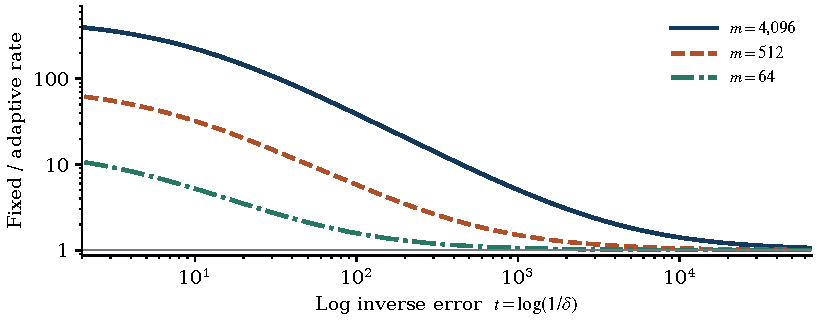
\includegraphics[width=.85\linewidth]{figures/confidence.pdf}
 \caption{Feedback gain as a function of the required confidence. Each curve shows \((m+t)/(\log m+t)\), the ratio in \cref{thm:samples} up to universal constants. The horizontal coordinate is \(t=\log(1/\delta)\). Both axes are logarithmic.}\label{fig:regimes}
\end{figure}

The worst-case rate hides a difference between the two answers. Let \(N_+\) and \(N_-\) be the respective infima of \(\sup_{A\in\Aplus}\E_A\tau\) and \(\sup_{A\in\Aminus}\E_A\tau\) over adaptive tests that meet the error requirement on both classes and have finite worst-case expected cost.

\begin{theorem}[Cost on each sign]\label{thm:classwise}
One test simultaneously attains the two minimax expected costs, up to universal constants,
\[
 N_+=\Theta\!\left(\frac{m^2\log m+t}{\gamma^2}\right),\qquad
 N_-=\Theta\!\left(\frac{m^2(\log m+t)}{\gamma^2}\right).
\]
On every run its cost is at most \(C m^2(\log m+t)/\gamma^2\).
\end{theorem}

Both signs require an initial search. On a positive input, the algorithm can extract a unit vector \(v\) with \(v^\top A v\ge\gamma/48\) at constant success probability. Fresh measurements along \(vv^\top\) can then validate that direction. The proof in \cref{sec:classwise} turns this observation into a single stopping rule for both signs.

\begin{theorem}[Number of feedback batches]\label{thm:rounds}
There are universal constants \(c,C>0\) such that for every \(R\ge1\),
\[
 N_R(m,\gamma,1/8)\ \ge\ c\,e^{-CR}\frac{m^3}{\gamma^2}.
\]
In particular every fixed number of batches has cost \(\Theta_R(m^3/\gamma^2)\). For fixed \(\varepsilon>0\), any family of tests with cost \(O(m^{3-\varepsilon}/\gamma^2)\) needs \(\Omega_\varepsilon(\log m)\) batches.
\end{theorem}

The sample-optimal adaptive test below uses \(O(\log m\max\{1,(m/(\log m+t))^{1/4}\})\) batches. For \(t\ge m\), the one-batch design already attains the optimal worst-case sample rate. Determining the least number of batches that attains \eqref{eq:ad} on the full matrix class remains open in the fixed-risk regime.

\paragraph{How the sign enters the lower bound.}
The difficult instances share a Gaussian matrix drawn once at the start of the experiment. On the positive side a rank-one perturbation competes with this background. Repeating a query averages away its observation noise while preserving the contribution of the background. For a fixed design one can whiten the entire response vector. With feedback the design itself depends on the unknown perturbation. We control how fast the transcript acquires information about its two factors, then translate that control into a bound on the distance between the positive and negative transcript laws. This last step matters because a test can in principle identify the sign while learning little about either factor.

\paragraph{Connections to earlier work.}
The change of variables \(M=-A-\gamma I\) maps the negative class to a positive semidefinite matrix and the positive class to \(\lambda_{\min}(M)\le-2\gamma\). Needell, Swartworth and Woodruff~\cite{needell2022} established adaptive and nonadaptive separations for positive semidefiniteness testing with exact queries. Their Theorem~31 and Remark~32 use the shifted dilation of a spiked Gaussian matrix and draw on the sketching lower bound of Li and Woodruff~\cite{li2016}. We use that family here. With fresh noise and repeated queries, the squared eigenvalues of a contracted design Gram matrix determine the fixed-design mixture bound. Nenadov and Verlinde~\cite{nenadov2026} study a complementary access model in which a random principal submatrix reveals a violation when the input is sufficiently far from the positive semidefinite cone in normalized Frobenius distance.

Feedback also changes the complexity of recovering a principal subspace from exact matrix--vector products~\cite{simchowitz2018}, recovering low-rank matrices under orthonormal sensing designs~\cite{kacham2024}, and identifying a nearly optimal arm in a linear bandit~\cite{maiti2026}. Here a matrix--vector product already costs \(m\) scalar measurements. The output is one bit, and the alternative allows a full-rank matrix with an unknown leading eigenspace. A lower bound for recovering that eigenspace would require an additional reduction to apply to this decision problem.

General-answer linear pure exploration gives an earlier explanation for the high-confidence asymmetry. For fixed \(m,\gamma\), the characteristic time of Degenne et al.~\cite{degenne2020} on a spanning design containing a fine net of rank-one directions has worst-case order \(\gamma^{-2}\) on positive inputs and \(m^2\gamma^{-2}\) on negative inputs. A near-maximizing direction separates a positive input from every negative one. On a negative input, uniform basis measurements suffice, and the spherical average in \eqref{eq:sph} gives the matching obstruction. Their asymptotic result holds as \(\delta\) tends to zero with the design fixed. \Cref{thm:classwise} identifies the discovery cost and gives rates uniform in all three parameters.

On the algorithmic side, the second-moment estimate of Gu et al.~\cite{gu2026} already leads to an \(O(m^2\log^2m/\gamma^2)\) fixed-risk test in this model. We give the reduction in \cref{sec:oja}. Our construction rescales the spectrum using a coarse estimate, in the spirit of absolute-value preconditioning~\cite{vecharynski2013}, and implements a block Chebyshev recurrence with noisy scalar probes. Under the null a quadratic energy controls its upper tail. Under the alternative an inverse moment of the growing component controls its lower tail. These two estimates give the additive \(\log m+\log(1/\delta)\) dependence in \eqref{eq:ad}.

\section{Confidence and fixed designs}\label{sec:fixed}

Two elementary experiments account for the \(t\) and \(m\) terms of the fixed-design rate. The first measures a directional contrast against a scalar null. The second measures an orthonormal basis of the symmetric matrices.

\begin{proposition}[Cost of confidence]\label{prop:confidence}
For every \(\delta\)-correct test, some negative input satisfies
\(\E_A\tau\ge c m^2\log(1/\delta)/\gamma^2\) for a universal \(c>0\).
\end{proposition}
\begin{proof}
Take \(A_0=-2\gamma I_m\). For each unit \(u\) put
\[
 A_u=A_0+\alpha(uu^\top-I_m/m),\qquad
 \alpha=\frac{3\gamma}{1-1/m}.
\]
Then \(\lambda_{\max}(A_u)=\gamma\) and
\(\|A_u\|_F^2=4m\gamma^2+9\gamma^2/(1-1/m)\le1\).
For a fixed \(u\), the Gaussian chain rule for the stopped likelihood and data processing to the final sign give
\[
 \frac{\alpha^2}2\,\E_0\sum_{j=1}^{\tau}
 \left(u^\top Q_j u-\tr(Q_j)/m\right)^2
 \ \ge\ \kl(\delta,1-\delta).
\]
Here \(\kl\) is binary relative entropy. To obtain the stopped identity, pad the experiment after stopping with zero queries, apply the chain rule at a deterministic horizon, and pass to the increasing limit of the transcript sigma fields. We may assume the worst-case mean stopping time is finite. Under \(A_0\) the entire policy is independent of an auxiliary uniform unit vector \(u\). Its fourth moments satisfy
\(\E[u_i u_j u_k u_l]=(\delta_{ij}\delta_{kl}+\delta_{ik}\delta_{jl}+\delta_{il}\delta_{jk})/[m(m+2)]\)
by rotational invariance and \(\|u\|=1\). Thus
\begin{equation}\label{eq:sph}
 \E_u (u^\top Qu-\tr Q/m)^2
 =\frac{2}{m(m+2)}
    \left(\|Q\|_F^2-\frac{(\tr Q)^2}{m}\right)
 \le\frac{2}{m(m+2)} .
\end{equation}
For example, $Q=I/\sqrt m$ spends its entire energy on trace and has zero contrast in \eqref{eq:sph}. More generally $(\tr Q)^2\le \operatorname{rank}(Q)\|Q\|_F^2$ by Cauchy--Schwarz on the nonzero eigenvalues. The Lean supplement contains a proof of this trace bound for real square matrices.

Averaging the preceding likelihood bound, using \(\alpha\le6\gamma\) and \(\kl(\delta,1-\delta)=(1-2\delta)\log((1-\delta)/\delta)\), proves the claim.
\end{proof}

\begin{lemma}[Reconstruction in one batch]\label{lem:reconstruct}
There is a fixed design of cost \(O(m^2[m+\log(1/\delta)]/\gamma^2)\) returning \(\widehat A\) with \(\|\widehat A-A\|_{\op}\le\gamma/2\) with probability at least \(1-\delta\).
\end{lemma}
\begin{proof}
Query each of the \(D=m(m+1)/2\) matrices of a Frobenius-orthonormal basis \(k\) times. The error \(E\) obtained by averaging the basis coordinates has independent \(\N(0,1/k)\) coordinates in this basis. Every unit \(u\) therefore gives \(u^\top E u\sim\N(0,1/k)\). A \(1/4\)-net of the sphere has size at most \(9^m\) and \(\|E\|_{\op}\le2\max_{u\ \mathrm{in\ net}}|u^\top E u|\). The failure probability is at most \(2\cdot9^m\exp(-k\gamma^2/32)\). Take \(k=\lceil32[m\log9+\log(2/\delta)]/\gamma^2\rceil\). On the success event Weyl's inequality gives the correct sign.
\end{proof}

\paragraph{What a fixed design can see.}
We give the mixture argument since it identifies the statistic of a noisy design that controls distinguishability. Write \(d=\lfloor m/2\rfloor\), and set
\[
 \sigma=\gamma/(16\sqrt d),\qquad a=128/\sqrt d,\qquad
 A_i=-2\gamma I_m+\sigma\dil(G+i aUV^\top),\quad i\in\{0,1\}.
\]
The entries of \(G\in\R^{d\times d}\) and of \(U,V\in\R^d\) are independent standard Gaussians. The symmetric dilation has off-diagonal blocks \(X,X^\top\) and vanishing diagonal blocks, padded by a zero coordinate for odd \(m\). \Cref{sec:discovery} shows that each prior can be restricted to its promised class at a cost of \(O(e^{-cd})\) in total variation.

Fix the seed and the first \(n\) queries of a nonadaptive design. After removal of the known intercept, the null covariance is \(\Sigma=I+\sigma^2LL^\top\), where row \(j\) of \(L\) is the vectorization of \(2(Q_j)_{12}\). Each row has squared norm at most two. Whitening gives a standard Gaussian under the null and a Gaussian with conditional mean \(aFz\) and identity covariance under the alternative, where \(z=\vecop(UV^\top)\), \(F=\sigma\Sigma^{-1/2}L\). Put \(K=F^\top F\). If \(s_j\) are the eigenvalues of \(\sigma^2L^\top L\), then
\begin{equation}\label{eq:softGram}
 \kappa:=\tr K^2
   =\sum_j\left(\frac{s_j}{1+s_j}\right)^2
   \le\sum_j s_j \le 2\sigma^2n .
\end{equation}

To bound the mixture distance, suppose \(a^4\kappa\le10^{-4}\). The event \(E=\{\|Kz\|^2\le100\kappa\}\) has probability \(p\ge0.99\), since \(\E zz^\top=I\). Denote by \(P_{1,E}\) the mixture conditioned on \(E\) and by \(P_0\) the whitened null. For an independent copy \(z'\), the Gaussian likelihood identity gives
\[
 1+\chi^2(P_{1,E}\Vert P_0)
 =p^{-2}\E[\ind_E(z)\ind_E(z')\exp(a^2 z^\top K z')].
\]
For \(z\in E\) the matrix \(M=a^2\mat(Kz)\) satisfies \(\|M\|_F^2\le0.01\), where \(\mat\) inverts vectorization. Integrating over both Gaussian factors of \(z'\) gives \(\E_{z'}\exp(a^2z^\top Kz')=\det(I-M^\top M)^{-1/2}\le(1-\|M\|_F^2)^{-1/2}\). Discarding \(\ind_E(z')\) yields \(1+\chi^2\le0.99^{-3/2}\). Restoring the excluded mass, the unconditioned transcript distance is at most \(0.01+\tfrac12\sqrt{0.99^{-3/2}-1}<0.1\).

By \eqref{eq:softGram} this applies whenever \(n\le c_0d^3/\gamma^2\) for a universal \(c_0>0\). The same priors work for every seed. Averaging over the seed and restricting to the promised classes gives distance less than \(1/4\) for all sufficiently large \(d\). A test of worst-case expected cost \(B\) can be truncated at \(\lceil8B\rceil\) with additional error at most \(1/8\). Its two output laws would have distance at least \(1/2\). This proves \(B=\Omega(m^3/\gamma^2)\), with the bounded dimensions covered by \cref{prop:confidence}. Taking the maximum with the confidence bound and using \cref{lem:reconstruct} proves \eqref{eq:na}.

\section{An adaptive test with a deterministic budget}\label{sec:algorithm}

The test measures a coarse approximation to the matrix and uses it to set the scale of a noisy Chebyshev iteration. On the negative class the iteration has a conserved quadratic energy in the absence of noise. A positive eigenvalue produces an expanding component. Several probe vectors, updated on a common scale, allow an inverse moment of this component to control the probability of missing it.

\begin{proposition}\label{prop:adaptive-algorithm}
Put \(L=\log(1024m)\) and \(T=\log(16/\delta)\). There is a test with error at most \(\delta\) on every promised matrix and a deterministic budget of at most
\[
 C\,m^2(L+T)/\gamma^2
\]
scalar observations. It uses at most \(1+C L\max\{1,(m/(L+T))^{1/4}\}\) batches, for a universal constant \(C\).
\end{proposition}

\paragraph{Setting the spectral scale.}
Choose \(b=\min\{m,L+T\}\), and define
\[
 \tau=\gamma\sqrt{m/b},\qquad \eta=\frac{\gamma}{\gamma+2\tau},
 \qquad k_0=\left\lceil 64b(1+T/m)/\gamma^2\right\rceil .
\]
Measure each member of a Frobenius-orthonormal basis of symmetric matrices \(k_0\) times in one batch. Coordinate averages give \(\widehat A=A+E\), with independent \(N(0,1/k_0)\) coordinates in this basis. For each unit vector \(u\), \(u^\top E u\) has variance \(1/k_0\). Approximating a top absolute Rayleigh direction by a point of a \(1/4\)-net of size \(9^m\) gives \(\|E\|_{\mathrm{op}}\le 2\max_{u\text{ in net}}|u^\top E u|\). Hence the event \(\mathcal G=\{\|E\|_{\mathrm{op}}\le\tau\}\) has
\[
 \Pr(\mathcal G^c)\le 2\cdot 9^m e^{-k_0\tau^2/8}\le e^{-T}.
\]
The test forms \(P=(|\widehat A|+\tau I)^{-1/2}\), where \(|\widehat A|\) has eigenvalues \(|\lambda_i(\widehat A)|\) in the eigenbasis of \(\widehat A\). Write \(C_A=PAP\). On \(\mathcal G\), the inequalities \(\pm A\preceq |\widehat A|+\tau I\) place its spectrum in \([-1,1]\). A negative input gives \(C_A\prec0\). For a positive input take \(Au=\lambda u\), \(\|u\|_2=1\), \(\lambda\ge\gamma\). Cauchy--Schwarz gives
\[
 u^\top|\widehat A|u\le\|\widehat A u\|_2\le\lambda+\tau .
\]
The Rayleigh quotient of \(C_A\) at \(P^{-1}u\) is therefore at least \(\lambda/(\lambda+2\tau)\ge\eta\). With \(\rho=1-\eta/2\), \(a=2-\eta\) and \(B=a C_A+\rho I\), the two cases now obey
\[
 \|B\|_{\mathrm{op}}\le\rho \quad\text{on the negative class},\qquad
 \lambda_{\max}(B)\ge 1+\eta \quad\text{on the positive class}.
\]
Here \(0<\eta\le 1/3\). The transform \(P\) is known after the first batch. All subsequent products involving \(C_A\) are measured.

\paragraph{A block update from scalar observations.}
Set
\[
 p=2\left\lceil\frac{T}{2L}\right\rceil,\quad s=p+2,\quad d=ms,\quad
 r=\left\lceil\frac{8L}{\sqrt\eta}\right\rceil,\quad
 k=\left\lceil\frac{256(d+2p)}{\tau^2\eta^{3/2}}\right\rceil .
\]
Start with \(X_{-1}=0\) and an \(m\times s\) matrix \(X_0\) of independent standard Gaussians drawn by the test. Given \(X=X_{j-1}\), put \(F=\|X\|_F\), \(v_h=X_{\cdot h}/F\) and \(k_h=\max\{1,\lceil k\|v_h\|_2^2\rceil\}\). Set \(v_h=0\) when \(F=0\). For \(i\le m\), \(h\le s\), let
\[
 W_{ih}=\tfrac12\big[(Pe_i)(Pv_h)^\top+(Pv_h)(Pe_i)^\top\big],
 \qquad \ell_{ih}=\|W_{ih}\|_F\le\|v_h\|_2/\tau .
\]
Measure \(W_{ih}/\ell_{ih}\) independently \(k_h\) times and multiply the average by \(\ell_{ih}\). This gives mean \(e_i^\top C_A v_h\) and variance \(\ell_{ih}^2/k_h\le1/(\tau^2k)\). For \(\ell_{ih}=0\), use zero queries and take the estimate zero. Add independent Gaussian noise to each estimate to bring its variance to \(1/(\tau^2k)\). Since \(\sum_h k_h\le k+s\), this costs at most \(m(k+s)\) scalar queries in one batch. Zero queries can pad each batch to that length.

Multiplying the resulting matrix of estimates by \(2aF\) and adding \(2\rho X_{j-1}-X_{j-2}\) implements the recursion
\begin{equation}\label{eq:upper-recurrence}
 X_j=2BX_{j-1}-X_{j-2}+\xi_j,\qquad
 \nu_j=\frac{4a^2\|X_{j-1}\|_F^2}{\tau^2 k}.
\end{equation}
Conditioned on the past, the entries of \(\xi_j\) are independent centered Gaussians of variance \(\nu_j\). In particular all columns have the same conditional noise scale even if their norms differ substantially. After \(r\) updates the test reports the positive class precisely when
\[
 S_r^2=\|X_r\|_F^2+\|X_{r-1}\|_F^2>H^2,\qquad
 H^2=\frac{2(d+2p)}{\eta}\exp(r\sqrt\eta/4).
\]

\paragraph{The negative class.}
Condition on any first-batch outcome in \(\mathcal G\). For \(m\times s\) matrices use the Frobenius inner product and define
\[
 D(x,y)=\|x\|_F^2+\|y\|_F^2-2\langle Bx,y\rangle .
\]
Expanding the squares gives \(D(2Bx-y,x)=D(x,y)\). Since \(\|B\|_{\mathrm{op}}\le\rho\),
\[
 D(x,y)\ge(1-\rho)(\|x\|_F^2+\|y\|_F^2),\qquad
 D(x,y)=\|Bx-y\|_F^2+\langle x,(I-B^2)x\rangle .
\]
Write \(D_j=D(X_j,X_{j-1})\). Given \(x=X_{j-1}\), \(y=X_{j-2}\), \(D=D_{j-1}>0\), the conditional law is
\[
 \frac{D_j}{D}\ \stackrel{\rm law}{=}\ 
 1-z^2+\|z e_1+\sqrt v\,g\|_2^2,\qquad
 z=\|Bx-y\|_F/\sqrt D\le 1,\quad
 v=\nu_j/D\le \frac{32}{\tau^2 k\eta},
\]
where \(g\sim N(0,I_d)\). This follows by rotating the vector of entries of \(Bx-y\). If \(D=0\), both matrices are zero and \(D_j=0\).

For \(Y=1-z^2+\|z e_1+\sqrt v\,g\|_2^2\) the moment-generating function near zero is
\[
 e^u(1-2vu)^{-d/2}\exp\!\left(\frac{2vz^2 u^2}{1-2vu}\right).
\]
Every Taylor coefficient increases weakly with \(z^2\), so the \(p\)th moment is largest at \(z=1\). For that value the Gaussian moment expansion gives
\[
 \mathbb E Y^p
 =\sum_{j=0}^p\binom{p}{j}v^j
      \prod_{i=0}^{j-1}(d+2p-2-2i)
 \le [1+v(d+2p)]^p.
\]
Indeed, apply the polynomial heat operator \(\exp(v\Delta/2)\) to \(\|x\|^{2p}\) at \(e_1\), using \(\Delta\|x\|^{2q}=2q(d+2q-2)\|x\|^{2q-2}\). The choice of \(k\) gives \(v(d+2p)\le\sqrt\eta/8\). Since \(D_0\sim\chi_d^2\), \(\mathbb E D_0^p\le(d+2p)^p\). Iterating the conditional bound and using \(S_r^2\le2D_r/\eta\), we obtain
\[
 \Pr(S_r>H\mid\widehat A)
 \le \exp(-pr\sqrt\eta/8)\le e^{-pL}\le e^{-T}.
\]

\paragraph{The positive class.}
Fix any first-batch outcome in \(\mathcal G\) and let \(w\) be a top unit eigenvector of \(B\) with eigenvalue \(\beta\). Put \(\alpha=\operatorname{arcosh}\beta\), so that \(\alpha\ge\sqrt\eta\) by \(\cosh(\sqrt\eta)\le1+\eta\). The projected difference \(z_j=w^\top X_j-e^{-\alpha}w^\top X_{j-1}\) satisfies
\[
 z_j=e^\alpha z_{j-1}+\sqrt{\nu_j}\,g_s,\qquad g_s\sim N(0,I_s)
\]
conditionally on the past, since \(e^\alpha+e^{-\alpha}=2\beta\).

The reason for choosing \(s=p+2\) appears here. For \(g_s\sim N(0,I_s)\), \(\mu\ne0\) and \(\sigma>0\), a Gaussian integration gives
\[
 \mathbb E\|\mu+\sigma g_s\|_2^{-p}
 =\frac{1}{\Gamma(p/2)}
    \int_0^{1/(2\sigma^2)}u^{p/2-1}e^{-u\|\mu\|_2^2}\,du
 \le \|\mu\|_2^{-p}.
\]
To see the identity, insert the Laplace integral for \(r^{-p}\) and substitute \(u=t/(1+2\sigma^2t)\) after integrating over \(g_s\). The powers of \(1+2\sigma^2t\) cancel because \(s=p+2\). The inequality extends to \(\sigma=0\) by equality. Thus
\[
 \mathbb E\|z_r\|_2^{-p}
 \le e^{-pr\alpha}\mathbb E\|z_0\|_2^{-p}
 =e^{-pr\alpha}\frac{2^{-p/2}}{\Gamma(1+p/2)}
 \le e^{-pr\alpha}(e/p)^{p/2},
\]
where all expectations condition on the coarse estimate. The finite initial inverse moment and this recursion also give zero probability of a vanishing projected difference. Since \(\|z_r\|_2\le\sqrt2 S_r\), Markov's inequality gives
\[
 \Pr(S_r\le H\mid\widehat A)
 \le [H\sqrt{2e/p}\,e^{-r\alpha}]^p \le e^{-T}.
\]
For the last step, \(d+2p\le3mp\), \(\eta^{-1}\le 3\sqrt m\), and
\(\sqrt{12em/\eta}\le e^L\), whereas \(r\sqrt\eta\ge8L\).
Adding \(\Pr(\mathcal G^c)\) gives error at most \(2e^{-T}\le\delta\) on either class.

\paragraph{Counting observations.}
The exact padded budget is
\[
 \frac{m(m+1)}2\,k_0 + m(k+s)r .
\]
The first term is \(O(m^2(b+T)/\gamma^2)\) since \(b\le m\). In the second term use \(d+2p\le3mp\), \(s\le2p\), \(r\le 9L/\sqrt\eta\), and \(\tau\eta\ge\gamma/3\). The part of \(k\) before rounding contributes \(O(m^2pL/\gamma^2)\). Rounding and the extra \(s\) queries per row cost \(O(mpL/\sqrt\eta)\), absorbed by the same bound since \(\eta^{-1}\le3\sqrt m\) and \(\gamma\le1\). Finally \(pL\le T+2L\), \(b\le L+T\), and \(1/\sqrt\eta\le\sqrt3(m/b)^{1/4}\). These estimates give both bounds of Proposition~\ref{prop:adaptive-algorithm}.

\section{The cost of discovering the spectral sign}\label{sec:discovery}

We prove that for some absolute \(c>0\), every test with error at most
\(1/8\) on each input has worst-case expected cost at least
\(c m^2\log(m)/\gamma^2\).
A rank-one perturbation changes the answer even when its two factors
remain largely unknown. We bound the distance between the two
\emph{observation laws} through the posterior mean of their common
Gaussian background. This proves a lower bound for the decision itself.

\subsection{Two matrix priors and the information in their factors}

Put \(d=\lfloor m/2\rfloor\), \(\beta=128\),
\(\sigma=\gamma/(16\sqrt d)\), \(a=\beta/\sqrt d\), and
\(\theta=\sigma a=8\gamma/d\). Draw independent standard Gaussian
vectors \(U,V\in\mathbb R^d\) and a matrix \(G\in\mathbb R^{d\times d}\)
with independent standard Gaussian entries. Write
\(\mathcal D(B)=\bigl(\begin{smallmatrix}0&B\\ B^\top&0\end{smallmatrix}\bigr)\),
with a zero row and column appended when \(m\) is odd. Under
law \(P_i\), \(i\in\{0,1\}\), the unknown matrix is
\[
 A_i=-2\gamma I_m+\sigma\mathcal D(G+i a UV^\top).
\]
We use the full Gaussian priors until the last step of the proof.
Given a symmetric query \(Q\), take \(D=2Q_{12}\) from its two
\(d\)-dimensional blocks. Removing the known shift from the answer gives
\begin{equation}\label{eq:disc-observation}
 Y=\sigma\langle D,G\rangle+i\theta U^\top D V+\xi,
 \qquad \|D\|_{\mathrm F}^2\le2,\qquad \xi\sim N(0,1).
\end{equation}
Fix a deterministic budget \(n\). After an early decision the algorithm
can fill out the transcript with zero queries. Let \(\mathcal H_j\)
denote its seed and the first \(j\) responses.

\begin{lemma}\label{lem:disc-information}
Under \(P_1\), let
\(S_j=I(U;\mathcal H_j\mid V,G)+I(V;\mathcal H_j\mid U,G)\).
Then \(S_n\le \exp(256\gamma^2 n/d^2)-1\).
\end{lemma}

\begin{proof}
Write the two summands as \(J_U(j)\) and \(J_V(j)\).
For fixed \(V,G\) the likelihood along the realized history is a product
of Gaussian densities linear in \(U\) in their means. The query at each
step is specified by the preceding responses and seed. Completing the
square gives conditional covariance
\[
 C_{U,j}=\Big[I+\theta^2\sum_{\ell=1}^j
       (D_\ell V)(D_\ell V)^\top\Big]^{-1}\preceq I.
\]
For \(D=D_{j+1}\), the Gaussian channel in the next scalar answer therefore
increases \(J_U\) by
\(\tfrac12\mathbb E_1\log(1+\theta^2(DV)^\top C_{U,j}DV)\).
To bound this quantity with \(D\) chosen from the data, apply the entropy
variational inequality conditionally on \(\mathcal H_j\). For fixed \(D\)
and any law \(\rho\) with relative entropy \(r\) to \(N(0,I_d)\),
\[
 \mathbb E_\rho\|DV\|^2
 \le 2\|D\|_{\mathrm F}^2+4\|D\|_{\mathrm{op}}^2r.
\]
Indeed, for \(D\ne0\) use \(\lambda=(4\|D\|_{\mathrm{op}}^2)^{-1}\):
the Gaussian log moment generating function at \(\lambda\) is
\(-\tfrac12\log\det(I-2\lambda D^\top D)
 \le 2\lambda\|D\|_{\mathrm F}^2\). The zero query gives the inequality directly.
For \(\rho=\mathcal L_1(V\mid\mathcal H_j)\), the expected entropy is
\(I(V;\mathcal H_j)\le J_V(j)\), by independence of \(V\) from \((U,G)\).
It follows that
\(J_U(j+1)-J_U(j)\le2\theta^2+4\theta^2J_V(j)\).
The same argument with \(D^\top\) interchanges \(U\) and \(V\).
Thus \(1+S_{j+1}\le(1+4\theta^2)(1+S_j)\), starting at \(S_0=0\).
\end{proof}

\subsection{A bound on the distance between the transcript laws}

Identify matrices with vectors by a fixed vectorization, and set
\(g=\operatorname{vec}(G)\), \(z=\operatorname{vec}(UV^\top)\).
During the \(j\)th unit interval take \(q_t=\operatorname{vec}(D_j)\)
and observe
\[
 dY_t=\sigma q_t^\top (g+i a z)\,dt+dW_t,\qquad j-1<t\le j.
\]
The original strategy reads the unit increments. Conditional on these
increments and the seed, the extra paths are independent standard
Brownian bridges translated by the linear interpolants. They carry no
further information at time \(n\). Denote the enlarged observed
filtration by \(\mathcal F_t\). In what follows \(P_i^t\) is the law
on this filtration up to time \(t\), also for a bounded stopping time.

Introduce the matrices and vector
\begin{align*}
 K_t&=\sigma^2\int_0^t q_s q_s^\top ds,&
 C_t&=(I+K_t)^{-1},& T_t&=I-C_t,\\
 s_t&=\sigma\int_0^t q_s\,dY_s,&
 \mu_t&=C_t s_t,& F_t&=\sigma q_t^\top C_t .
\end{align*}
Matrix differentiation gives \(dT_t=F_t^\top F_t\,dt\).
In particular \(0\preceq T_t\preceq I\) and
\(\operatorname{tr}T_t\le\operatorname{tr}K_t\le k\), where
\(k=2\sigma^2n\). For a fixed latent vector \(h=g+i a z\), the
likelihood relative to a Wiener observation is
\[
 L_t(h)=\exp(h^\top s_t-\tfrac12 h^\top K_t h).
\]
For fixed \(h\) its drift has squared integral bounded by
\(2n\sigma^2\|h\|^2\), so the exponential is a true martingale up to \(n\).
Integration over the prior gives the mixture likelihood, including at
bounded observation stopping times. Under \(P_0\) the posterior mean of
\(g\) is \(\mu_t\). Under \(P_1\), completing the square in \(g\)
at fixed \(U,V,\mathcal F_t\) gives the conditional law
\(N(\mu_t-aT_t z,C_t)\). Consequently the predictive drift of \(Y\)
under \(P_1\) exceeds that under \(P_0\) by
\begin{equation}\label{eq:disc-drift}
 b_t=aF_t\,\mathbb E_1[z\mid\mathcal F_t].
\end{equation}
Subtracting each law's predictive drift gives an observed Brownian
innovation: the resulting continuous martingale has quadratic variation \(t\).
The likelihood ratio of the two positive mixture densities has stochastic
logarithm \(b_t\) against the null innovation. Indeed, relative to Wiener measure each positive mixture likelihood has a stochastic logarithm by Brownian martingale representation. Girsanov's theorem and uniqueness of the observed drift identify its integrand with the posterior mean drift. The quotient rule then gives the stated stochastic logarithm.
For the observed stopping times \(\tau\le n\) this yields
\begin{equation}\label{eq:disc-KL}
 D_{\mathrm{KL}}(P_1^\tau\Vert P_0^\tau)
   =\tfrac12\mathbb E_1\int_0^\tau b_t^2\,dt .
\end{equation}
The stochastic integral in the alternative log likelihood is integrable,
since conditional Jensen and \(T_n\preceq I\) bound
\(\mathbb E_1\int b_t^2dt\le a^2\mathbb E_1[z^\top T_nz]
\le a^2d^2\).

The following decomposition gives a sharper estimate close to the
start of the experiment. Define two matrix-valued martingales
\[
 \widehat G_t=\mathbb E_1[G\mid\mathcal F_t],\qquad
 M_t=\mathbb E_1[G(VV^\top-I)\mid\mathcal F_t].
\]
They start at zero and are square integrable. They have continuous
versions: their Wiener posterior numerators and the strictly positive
denominator are continuous martingales, conditional on the independent
seed. Gaussian integration by parts in \(U_i\) and then in each \(G_{i\ell}\)
gives
\begin{equation}\label{eq:disc-Stein}
 \mathbb E_1[UV^\top\mid\mathcal F_t]=a(\widehat G_t+M_t).
\end{equation}
In detail, along a fixed path
\(\partial_{U_i}L_t=a\sum_\ell V_\ell\partial_{G_{i\ell}}L_t\).
Multiply by \(V_j\), integrate against the prior and divide by its
likelihood. The two integration-by-parts identities give, respectively,
the conditional moments of \(U_iV_j\) and
\(a\sum_\ell G_{i\ell}V_\ell V_j\). To justify the operations, note
that \(s_t\) belongs to the range of \(K_t\) because the directions are
piecewise constant. Thus \(L_t\) is bounded as a function of \(h\) on
each realized path. Its first derivatives are bounded there by a
path-dependent constant times a polynomial in the latent variables.
The same argument applies along a stopped path.

For a bounded stopping time \(\tau\), total conditional variance gives
\(\operatorname{Cov}_1(g\mid\mathcal F_\tau)\succeq C_\tau\).
Subtracting the trace of this inequality from the prior variance yields
\(\mathbb E_1\|\widehat G_\tau\|_{\mathrm F}^2\le \mathbb E_1\operatorname{tr}T_\tau\le k\).
Also, for any continuous square-integrable vector martingale \(X\) starting
at zero under \(P_1\),
\begin{equation}\label{eq:disc-energy}
 \mathbb E_1\int_0^\tau |F_t X_t|^2dt\le\mathbb E_1\|X_\tau\|^2 .
\end{equation}
Indeed, apply It\^o's formula to \(X_t^\top C_t X_t\) using
\(dC_t=-F_t^\top F_t\,dt\). The terminal quadratic form is nonnegative
and the expected quadratic-variation term
\(\mathbb E_1\int_0^\tau\operatorname{tr}(C_t\,d\langle X\rangle_t)\)
is at most \(\mathbb E_1\|X_\tau\|^2\). Stopping first on a bounded
ball and passing to the limit justifies the expectation.
If \(\tau\) stops \(M\) when \(\|M_t\|_{\mathrm F}\) first reaches \(L>0\),
or at \(n\) if it does not, equations
\eqref{eq:disc-drift}--\eqref{eq:disc-energy} give
\begin{equation}\label{eq:disc-stop}
 D_{\mathrm{KL}}(P_1^\tau\Vert P_0^\tau)
 \le a^4(k+L^2).
\end{equation}

It remains to bound the probability of reaching \(L\).
For any law \(\rho\) with entropy \(r\) relative to \(N(0,I_d)\),
write \(S_\rho=\mathbb E_\rho VV^\top\). We have
\begin{equation}\label{eq:disc-coventropy}
 \|S_\rho-I\|_{\mathrm F}\le2\sqrt r+4r .
\end{equation}
The Gaussian maximizes entropy at a given second moment, so
\(\sum_j f(\lambda_j(S_\rho))\le2r\), with \(f(x)=x-1-\log x\).
Here finite relative entropy gives a finite second moment by the
Gaussian moment generating function. The scalar inequality
\(|x-1|\le\sqrt{2f(x)}+2f(x)\) follows by integrating \(f'\)
on either side of one, using \(f(x)\ge (1-x)^2/2\) below one and
\(f(x)\ge(x-1)^2/(2x)\) above one. Taking the Euclidean norm of
these eigenvalue bounds proves \eqref{eq:disc-coventropy}.

Take \(\rho=\mathcal L_1(V\mid G,\mathcal F_n)\). Its expected relative
entropy is \(I(V;\mathcal F_n\mid G)\le J_V(n)\le S_n\). On
\(\|G\|_{\mathrm{op}}\le8\sqrt d\), condition first on \(G,\mathcal F_n\)
and use \eqref{eq:disc-coventropy} and Jensen's inequality. The
complement costs at most
\[
 (d+\sqrt d)\,\mathbb E[\|G\|_{\mathrm{op}}
             \mathbf 1_{\{\|G\|_{\mathrm{op}}>8\sqrt d\}}],
\]
since \(V\) is independent of \(G\) before observing \(Y\).
A \(1/4\)-net on each unit sphere has size at most \(9^d\), giving
\(\Pr(\|G\|_{\mathrm{op}}>x)\le2\cdot9^{2d}e^{-x^2/8}\).
Integrating above \(8\sqrt d\) shows, for absolute \(c,C>0\),
\[
 \mathbb E_1\|M_n\|_{\mathrm F}
 \le 16\sqrt{dS_n}+32\sqrt d\,S_n+C d^{3/2}e^{-cd}
 =:B_n .
\]

Doob's maximal inequality gives \(P_1(\tau<n)\le B_n/L\).
For each test function \(0\le f\le1\) on the full transcript,
\(f_\tau=\mathbb E_0[f\mid\mathcal F_\tau]\) equals \(f\) on
\(\{\tau=n\}\) under both equivalent path laws. Hence
\(|\mathbb E_1f-\mathbb E_0f|\le P_1(\tau<n)+
 |\mathbb E_1 f_\tau-\mathbb E_0 f_\tau|\).
Pinsker's inequality and \eqref{eq:disc-stop} give the desired
transcript bound
\begin{equation}\label{eq:disc-finalTV}
 \|P_1^n-P_0^n\|_{\mathrm{TV}}\le \frac{B_n}{L}
                 +a^2\sqrt{(k+L^2)/2}.
\end{equation}

\subsection{Restriction to the promised classes and expected cost}

Take \(n\le d^2\log(d)/(4096\gamma^2)\) and \(L=d^{3/4}\).
Lemma~\ref{lem:disc-information} gives \(S_n\le d^{1/16}\), and
\(k\le d\log(d)/2^{19}\). The first term of \eqref{eq:disc-finalTV}
is \(O(d^{-3/16})\), the second \(O(d^{-1/4}+\sqrt{\log(d)/d})\).
Thus the total variation is at most \(1/8\) for all \(d\) larger than
an absolute constant, uniformly in \(\gamma\) and in the test.

Condition the null prior on \(\|G\|_{\mathrm{op}}\le8\sqrt d\) and
\(\|G\|_{\mathrm F}\le2d\). Under the alternative require these same events
and \(\sqrt{d/2}\le\|U\|,\|V\|\le2\sqrt d\).
The net bound just proved and the Gaussian chi-square tail bounds show
that the removed prior mass is \(O(e^{-c d})\) in each case.
On these events \(\|\sigma G\|_{\mathrm{op}}\le\gamma/2\) and
\(4\gamma\le\|\theta UV^\top\|_{\mathrm{op}}\le32\gamma\).
The maximal eigenvalue of the dilation equals the largest singular
value of its off-diagonal block. Consequently \(A_0\) has top
eigenvalue at most \(-3\gamma/2\), and that of \(A_1\) is at least
\(3\gamma/2\). Both matrices obey \(\|A_i\|_{\mathrm{op}}<35\gamma\).
Moreover, the shift is Frobenius-orthogonal to the dilation, so
\[
 \|A_i\|_{\mathrm F}^2
 \le 4m\gamma^2+4\sigma^2\|G\|_{\mathrm F}^2
                  +4i\theta^2\|U\|^2\|V\|^2
 \le (4m+d/16+4096)\gamma^2\le1
\]
for all sufficiently large \(d\).
Conditioning a prior costs its excluded mass in total variation, and
a common observation kernel contracts this distance. The two legal
transcript laws are therefore within \(1/4\) of one another for large \(d\).

Suppose now that the worst-case expected cost on legal inputs is \(B\).
Truncating the procedure at \(n=\lceil32B\rceil\) increases its
per-input error to at most \(5/32\). Its positive-decision probabilities
on the two legal mixtures must differ by at least \(11/16\). This
contradicts the preceding bound whenever
\(\lceil32B\rceil\le d^2\log(d)/(4096\gamma^2)\).
It follows that \(B\ge c m^2\log(m)/\gamma^2\) for all sufficiently
large \(m\). For the remaining dimensions \(\log m\) is bounded by an
absolute constant, and Proposition~\ref{prop:confidence} at error
\(1/8\) gives the same conclusion with a smaller \(c\).
Finally, a test with any error \(\delta\le1/8\) also satisfies this
fixed-error bound. Taking its maximum with Proposition~\ref{prop:confidence}
gives \(B\ge c' m^2(\log m+\log(1/\delta))/\gamma^2\).


\section{The cost on each side of the test}\label{sec:classwise}

A direction \(v\) with a positive Rayleigh quotient can be checked by repeated measurements of \(vv^\top\). The issue is how to find such a direction when the positive eigenspace could be one-dimensional. The block iteration in Section~\ref{sec:algorithm} provides one at the same cost as fixed-error testing.

\paragraph{Extracting a direction.}
Use the coarse estimate and recursion of Section~\ref{sec:algorithm} with \(b=1\), \(T=\log 128\), \(p=2\), \(s=4\), \(d=4m\), and increase \(k\) to \(\lceil 2^{18}d/(\tau^2\eta^{3/2})\rceil\). Keep the span \(K_j\) of the columns of \(X_0,\ldots,X_j\). We claim that for every positive input, with probability at least \(15/16\) the following procedure returns a unit \(v\) with \(v^\top A v\ge\gamma/48\). The proof concerns a fixed first-batch realization in the good event \(\mathcal G\).

Let \(D_j=D(X_j,X_{j-1})\) be the energy from Section~\ref{sec:algorithm} and \(E_j\) the event that every unit \(x\in K_j\) has \(x^\top C_A x\le\eta/8\). These events are decreasing. On \(E_j\), the compression of \(B\) to \(K_j\) has spectrum in \([-\rho,1-\eta/4]\), since \(\rho+a\eta/8\le1-\eta/4\). Thus \(D_j\ge(\eta/4) S_j^2\), where \(S_j^2=\|X_j\|_F^2+\|X_{j-1}\|_F^2\).

On \(E_{j-1}\), write \(x=X_{j-1}\), \(y=X_{j-2}\), \(e=D_{j-1}\), and \(w=Bx-y\). We have \(\|w\|_F^2\le10S_{j-1}^2\le40e/\eta\) because \(\|B\|_{\rm op}\le3\), and \(\nu_j\le64e/(\tau^2 k\eta)\). Conservation of the noiseless energy gives \(D_j=e+2\langle \xi_j,w\rangle+\|\xi_j\|_F^2\). For \(e>0\), use \((-e-z)_+\le z^2/(4e)\) to bound the energy discarded when the span leaves \(E_j\). Conditional on the past,
\[
 \mathbb E[(D_j)_+]\le e+d\nu_j+\nu_j\|w\|_F^2/e
 \le (1+\sqrt\eta/64)e .
\]
The final inequality uses \(d\eta\ge1\) and the choice of \(k\). For \(e=0\) the two previous iterates vanish. Nesting and iteration yield \(\mathbb E[D_r\mathbf 1_{E_r}]\le d e^{r\sqrt\eta/64}\), starting from \(\mathbb E D_0=d\). Use the threshold \(H\) of Section~\ref{sec:algorithm}. Markov's inequality on \(E_r\) and the positive-class inverse-moment estimate, respectively, give
\[
 \Pr(E_r,\ S_r>H)\le2e^{-15r\sqrt\eta/64},\qquad
 \Pr(S_r\le H)\le e^{-2L}.
\]
The latter calculation uses \(p=2\) in the inverse-moment bound. Increasing \(k\) preserves the conditional isotropic noise required there. Since \(r\sqrt\eta\ge8L\), these errors sum to less than \(1/128\). On \(E_r^c\), some unit \(x\in K_r\) satisfies \(x^\top C_A x>\eta/8\). The unit vector along \(Px\) has Rayleigh quotient exceeding \(\tau\eta/8\ge\gamma/24\).

The algorithm computes an orthonormal basis \(V\) of \(P K_r\). In the zero-dimensional case return a fixed unit vector. Otherwise, with \(h=\dim(P K_r)\), measure \(VFV^\top\) for each member \(F\) of a Frobenius-orthonormal basis of symmetric \(h\times h\) matrices. These queries have unit norm. Using fresh responses and \(O(h/\gamma^2)\) repetitions per member, the net estimate of Section~\ref{sec:algorithm} gives an estimate of \(V^\top A V\) within \(\gamma/96\) in operator norm with conditional probability at least \(127/128\). Lift a top unit eigenvector of the estimate by \(V\). Its Rayleigh quotient loses at most \(2\gamma/96\). The coarse estimate, the span test in the analysis, and the compression contribute total failure at most \(3/128\). The recursion costs \(O(m^2 L/\gamma^2)\) even with the increased \(k\). Since \(h\le 4(r+1)=O(m^{1/4}L)\), the compression costs \(O(h^3/\gamma^2)=O(m^2 L/\gamma^2)\), using \(L^2=O(m^{5/4})\). These are deterministic cost bounds on both classes.

\paragraph{Validation and stopping.}
On attempt \(j\ge1\), run a fresh copy of the direction procedure. Validate its output \(v\) by averaging \(n_j=\lceil c\gamma^{-2}\log(1/\epsilon_j)\rceil\) new responses to \(vv^\top\), with \(\epsilon_j=\delta/[16(j+1)^2]\). Accept the positive class if the average exceeds zero, and otherwise repeat. For an absolute \(c\) large enough, a Gaussian tail bound gives conditional false acceptance probability at most \(\epsilon_j\) on every negative input. On a positive input each attempt succeeds with conditional probability at least \((15/16)(1-\epsilon_j)>7/8\). Thus the expected cost on a positive input is bounded by
\[
 \sum_{j\ge1}8^{1-j}\big[O(m^2 L/\gamma^2)+n_j\big]
     =O((m^2 L+t)/\gamma^2).
\]
Interleave this search, one observation at a time, with the deterministic-budget test of Proposition~\ref{prop:adaptive-algorithm} at risk \(\delta/2\). Output the first answer received. Each test reads its own independent measurements. Overall error on the negative class is at most \(\delta/2+\sum_j\epsilon_j\), and on the positive class at most \(\delta/2\). The cost is at most twice the deterministic budget, and on positive inputs it is also at most twice the search cost plus one.

\paragraph{Matching lower bounds.}
For either class let \(B_*\) be the expected cost of a given test in the worst case over that class. Truncate at \(\lceil32 B_*\rceil\) and return the opposite class on timeout. The sum of the two worst-case errors is at most \(2\delta+1/32\), by Markov's inequality on the class being timed. The legal-prior transcript bound of Section~\ref{sec:discovery} then forces \(B_*=\Omega(m^2\log(m)/\gamma^2)\) for all sufficiently large \(m\). For the positive confidence term, compare \(A_-=-\gamma I\) with \(A_+=-\gamma I+2\gamma uu^\top\) for a fixed unit \(u\). Both have Frobenius norm \(\gamma\sqrt m\). Each query contributes at most \(2\gamma^2\) to relative entropy in either direction. The stopped Gaussian chain rule and data processing for the answer give \(2\gamma^2\mathbb E_{A_+}\tau_{\rm stop}\ge\kl(1-\delta,\delta)\ge t/2\). Reversing the two points gives the same fixed-error lower bound on the other class, which covers the remaining bounded dimensions after adjusting the absolute constant. Proposition~\ref{prop:confidence} supplies the \(m^2t/\gamma^2\) negative-class bound. Taking the larger of the discovery and confidence bounds proves Theorem~\ref{thm:classwise}.

\section{Round complexity lower bounds}
\label{sec:rounds}

Within each batch, the list of measurements is fixed by the preceding observations. A useful prior must therefore remain hard after conditioning on a random list. We track the conditional law of two latent Gaussian factors together with the background matrix they perturb. The error of this approximation grows at most exponentially with the number of batches.

\subsection{Gaussian innovation representation}

Let $d=\lfloor m/2\rfloor$, $\beta=128$, $\sigma=\gamma/(16\sqrt d)$ and $a=\beta/\sqrt d$. Write $\dil(D)$ for the symmetric matrix with off-diagonal blocks $D,D^\top$ and zero diagonal blocks (padded by zero in odd ambient dimension). The two input matrices have the form $-2\gamma I_m+\sigma\dil(\mat(\theta_b))$, $b\in\{0,1\}$, with unconditioned priors
\[
 \theta_0=g_0,\qquad
 \theta_1=g_0+a z,\qquad
 g_0\sim\N(0,I_{d^2}),\quad z=\vecop(UV^\top).
\]
Here $U,V$ are independent $d$-dimensional standard Gaussians independent of $g_0$, and $\mat$ inverts vectorization on $d\times d$ matrices. All three draws are fixed throughout a run. After subtracting the known intercept $-2\gamma\tr Q$ in each response, batch $j$ is a linear observation of $\sigma\theta_b$ with design matrix $L_j$ and independent unit noise. A row of $L_j$ is $\vecop(2Q_{12})^\top$ and hence has squared norm at most two. With $\Gamma_0=I$ and $\mu_0=0$, define
\begin{align}
 \Omega_j&=I+\sigma^2L_j\Gamma_{j-1}L_j^\top,\notag\\
 y_j&=\Omega_j^{-1/2}(Y_j-\sigma L_j\mu_{j-1}),\notag\\
 F_j&=\sigma\Omega_j^{-1/2}L_j\Gamma_{j-1},
 \quad T_j=F_j^\top F_j,\label{eq:innovations}\\
 \Gamma_j&=\Gamma_{j-1}-T_j,\qquad
 \mu_j=\mu_{j-1}+F_j^\top y_j.\notag
\end{align}
Conditional on the latent factors and the previous transcript, the positive channel is
\[
 y_j=aF_jz+h_j,\qquad h_j\sim\N(0,I).
\]
The negative channel has standard Gaussian innovations. Gaussian conditioning gives the background kernel
\begin{equation}
 \mathcal L(g_0\mid U,V,H_j)
 =\N\bigl(\mu_j-a(I-\Gamma_j)z,\Gamma_j\bigr).
 \label{eq:background-kernel}
\end{equation}
The regression is conditional on the factors, so its form is independent of their mixing law.

Every batch satisfies
\begin{equation}
 0\preceq T_j\preceq I,\qquad
 \tr T_j\le\frac{\gamma^2n_j}{128d}.
 \label{eq:batch-energy}
\end{equation}
For a deterministic total cap $N$, write
\[
 q=\frac{\gamma^2N}{128d^3}.
\]
Then $\tr T_j/d^2\le q$ for every realized history.

\subsection{Auxiliary covariance process}

Augment the batch response to the path
$y_j(t)=t y_j+\operatorname{bridge}_j(t)$, $0\le t\le1$, using a standard Brownian bridge.
Conditional on the factors, this path has drift $aF_jz$.
The bridge is sampled independently of the endpoint and of all hidden variables. Write $H_j$ for the algorithm's private coins and the augmented paths through batch $j$. During a batch the observation filtration grows only by the path seen so far. The design itself uses only the coins and the preceding endpoints.

Let $E_{ji}=\dil(\mat((F_j)_i))/2$ on the factor space $\R^{2d}$, with $(F_j)_i$ the $i$th row in column form. In particular, $x^\top E_{ji}x=(F_j z)_i$ for $x=(U,V)$. In an auxiliary experiment
$\mathsf Q$, the factors have a centered Gaussian distribution with covariance $S$, initially $I_{2d}$. During batch $j$, evolve
\begin{align}
 \dd S_t&=2a\sum_i S_tE_{ji}S_t\dd W_{ji}(t),\notag\\
 \dd y_{ji}(t)&=a\tr(E_{ji}S_t)\dd t+\dd W_{ji}(t).
 \label{eq:physical-flow}
\end{align}
Given the observation history at a batch endpoint, draw the current factors from $\N(0,S)$ and attach the background kernel \eqref{eq:background-kernel}. This constructs a comparison law on observations and the current hidden state. Hidden draws and the coins used to generate them are integrated out of $H_j$. The covariance evolution is the Gaussian projection filter for a static quadratic observation~\cite{brigo1999}. The joint error estimate needed to concatenate batches is proved in \cref{app:projection}.

The quantities that control this comparison are
\[
 D(S)=\frac{\norm{S-I}_{\Frob}^2}{2d},
 \qquad \Phi_p(S)=\frac{\tr(S^p)}{2d},
\]
and the current batch energy
\[
 \kappa_j(S)=16a^4\sum_{i,k}
       [\tr(SE_{ji}SE_{jk})]^2.
\]
Choose $h>0$ and $K>1$. Freeze the covariance permanently at the first of the boundary hits
\[
 D(S)=1/4,\qquad \Phi_4(S)=K,\qquad \kappa_j(S)=h^2.
\]
After freezing, the output drift in \cref{eq:physical-flow} continues at the frozen covariance.

\begin{lemma}[Batched comparison]
\label{lem:batch-comparison}
Let $\bar\kappa=8\beta^4K\sqrt q<h^2$.
For the unconditioned transcript laws $P_0,P_1$ under a hard sample cap $N$,
\begin{align}
 \TV(P_1,P_0)
 \le{}&R\sqrt{3/32}\,h \notag\\
 &+R\left[
 4(e^{hR}-1)+\frac{e^{27\beta^2R}}{K}
       +\frac{R\bar\kappa e^{6h}}{h^2}
       \right]\label{eq:comparison-bound}\\
 &+\frac{\beta}{2}\sqrt{R(e^{hR}-1)}.\notag
\end{align}
This bound holds for adaptive, randomized designs satisfying \cref{eq:batch-energy}.
\end{lemma}

The first line of \cref{eq:comparison-bound} is the cost of replacing the joint observation and factor kernel within each batch. The second line pays for every freezing event. The last line bounds the divergence of the auxiliary observations from the negative experiment. In particular, it includes the mean caused by the cross-covariance of $U$ and $V$.

\subsection{Proof of the round lower bound}

Set
\begin{equation}
 h=\frac{2^{-16}}{\beta^2R^2},\qquad
 K=2^{10}R e^{27\beta^2R},\qquad
 q_R=2^{-114}\beta^{-16}R^{-14}e^{-54\beta^2R}.
 \label{eq:round-parameters}
\end{equation}
For $q\le q_R$, these choices give
$\bar\kappa\le2^{-12}h^2/R^2$.
Substitution in \cref{eq:comparison-bound} yields
\begin{equation}
 \TV(P_1,P_0)<3/512.
 \label{eq:round-tv}
\end{equation}
The parameter calculation appears in \cref{app:round-constants}.

For $d\ge128$, conditioning the two actual matrix priors on the spectral and Frobenius promises adds less than $0.02$ to their total variation distance (\cref{app:expected}). A test with risk $1/4$ on both classes would require distance at least $1/2$. Thus a deterministic cap $128q_Rd^3/\gamma^2$ is insufficient. Truncation of the stopping time, with the confidence lower bound for the small-dimensional cases, now gives
\begin{equation}
 N_R(m,\gamma,1/8)\ge c\,q_R m^3/\gamma^2 .
 \label{eq:explicit-round}
\end{equation}
The details are in \cref{app:expected}. Since $\beta=128$,
$q_R=2^{-226}R^{-14}e^{-884736R}$. Absorbing $R^{-14}$ into the exponential proves \cref{thm:rounds}. If a test uses at most $K_0 m^{3-\eta}(\log m)^s/\gamma^2$ queries in worst-case expectation, then
\[
 CR\ge\eta\log m-s\log\log m-\log(K_0/c')
\]
for absolute $c',C>0$. Every fixed $\eta>0$ therefore requires $R=\Omega_\eta(\log m)$ batches as $m$ grows.

\begin{thebibliography}{10}\small
\bibitem{brigo1999} D. Brigo, B. Hanzon and F. Le Gland.
Approximate nonlinear filtering by projection on exponential manifolds of densities.
\emph{Bernoulli} 5 (1999), 495--534. \href{https://doi.org/10.2307/3318714}{doi:10.2307/3318714}.
\bibitem{degenne2020} R. Degenne, P. Menard, X. Shang and M. Valko.
Gamification of pure exploration for linear bandits.
\emph{International Conference on Machine Learning}, PMLR 119, 2432--2442, 2020.
\href{https://proceedings.mlr.press/v119/degenne20a.html}{Proceedings version}.
\bibitem{gu2026} A. Gu, S. Kumar, K. Tian and C. Yang.
Gap-free streaming PCA beyond rank-one updates: near-optimal rates and applications to differential privacy.
\href{https://arxiv.org/abs/2609.26508}{arXiv:2609.26508}, 2026.
\bibitem{kacham2024} P. Kacham and D. P. Woodruff.
Lower bounds on adaptive sensing for matrix recovery.
\emph{Advances in Neural Information Processing Systems} 36, 2023.
\href{https://arxiv.org/abs/2311.17281}{arXiv:2311.17281}.
\bibitem{li2016} Y. Li and D. P. Woodruff.
Tight bounds for sketching the operator norm, Schatten norms, and subspace embeddings.
\emph{APPROX/RANDOM}, LIPIcs 60, 39:1--39:11, 2016.
\href{https://arxiv.org/abs/2202.09797}{Corrected version, arXiv:2202.09797}.
\bibitem{maiti2026} A. Maiti, Y. Xu and K. Jamieson.
On the power of adaptivity for \(\varepsilon\)-best arm identification in linear bandits.
\href{https://arxiv.org/abs/2605.15663}{arXiv:2605.15663}, 2026.
\bibitem{needell2022} D. Needell, W. Swartworth and D. P. Woodruff.
Testing positive semidefiniteness using linear measurements.
\emph{IEEE Symposium on Foundations of Computer Science}, 2022.
\href{https://arxiv.org/abs/2204.03782}{arXiv:2204.03782}.
\bibitem{nenadov2026} R. Nenadov and L. Verlinde.
Positive semidefiniteness of random submatrices.
\href{https://arxiv.org/abs/2611.25662}{arXiv:2611.25662}, 2026.
\bibitem{simchowitz2018} M. Simchowitz, A. El Alaoui and B. Recht.
Tight query complexity lower bounds for PCA via finite sample deformed Wigner law.
\emph{ACM Symposium on Theory of Computing}, 1249--1259, 2018.
\href{https://doi.org/10.1145/3188745.3188796}{doi:10.1145/3188745.3188796}.
\bibitem{vecharynski2013} E. Vecharynski and A. V. Knyazev.
Absolute value preconditioning for symmetric indefinite linear systems.
\emph{SIAM Journal on Scientific Computing} 35 (2013), A696--A718.
\href{https://doi.org/10.1137/120886686}{doi:10.1137/120886686}.
\end{thebibliography}

\appendix
\section{Joint Gaussian approximation for quadratic observations}
\label{app:projection}

We prove the within-batch comparison used in \cref{lem:batch-comparison}. The joint law includes the observed path and the factor that generates the next batch. Controlling the marginal distribution of observations alone would lose this dependence.

\subsection{A stopped covariance flow}

Let $x\sim\N(0,I_p)$, let $L_1,\ldots,L_n\in\Sym_p$, and let
\[
 q_i(x)=\tfrac12x^\top L_i x-c_i.
\]
Consider the path experiment
\begin{equation}
 \dd Y_i(t)=q_i(x)\dd t+\dd B_i(t),\qquad 0\le t\le1.
 \label{eq:quadratic-path}
\end{equation}
Conditional on $Y(1)=y$, its path is $ty+\operatorname{bridge}(t)$,
where the bridge is independent of $x,y$. Its posterior for $x$ is therefore the posterior from the original endpoint observation.

Under an auxiliary innovation law, set $C_0=I_p$ and
\begin{equation}
 \dd C_t=\sum_i C_tL_iC_t\dd W_i(t),\qquad
 m_i(C)=\tfrac12\tr(L_iC)-c_i,\qquad
 \dd Y_i(t)=m_i(C_t)\dd t+\dd W_i(t).
 \label{eq:generic-flow}
\end{equation}
Write
\[
 A_i=C^{1/2}L_iC^{1/2},\qquad
 R_{ij}(C)=\tr(L_iCL_jC),\qquad
 \kappa(C)=\sum_{i,j}R_{ij}(C)^2.
\]
Stop at an energy boundary $\kappa(C)=\rho$, an upper spectral boundary
$\norm C_{\op}=M$, or any additional specified stopping boundary.
The stopping time is infinity if no boundary is reached. After stopping, freeze $C$ and retain the output drift $m(C)$.
At time one, draw the auxiliary latent variable conditionally from $\N(0,C_{1\wedge\tau})$.

The stopped flow stays positive definite. On any positive-definite interval, It\^o's formula gives
\begin{equation}
 \dd C_t^{-1}
 =-\sum_iL_i\dd W_i(t)+\sum_iL_iC_tL_i\dd t.
 \label{eq:inverse-flow}
\end{equation}
While $\norm{C_t}_{\op}\le M$, the inverse has bounded sample paths on finite time intervals. Thus it cannot reach a zero covariance eigenvalue before an upper boundary. Local strong existence and freezing define the full process. The bounded output drift also permits the change between Wiener reference measure and the auxiliary observation measure.

\begin{lemma}[Energy and joint-kernel error]
\label{lem:projection}
For the stopped construction above, the drift and quadratic variation density of $\kappa$ satisfy
\begin{equation}
 b_\kappa\le6\kappa^{3/2},\qquad
 \frac{\dd\ip{\kappa}{\kappa}_t}{\dd t}\le16\kappa^{5/2}.
 \label{eq:kappa-generator}
\end{equation}
Let $P$ be the joint law of the true path \eqref{eq:quadratic-path} and its latent variable, and let $\widetilde P$ be the auxiliary joint endpoint law. If $\kappa(C_t)\le\rho$ before stopping, then
\begin{equation}
 \TV(P,\widetilde P)
 \le\sqrt{3\rho/32}+\Prob_{\mathrm{aux}}(\tau\le1).
 \label{eq:joint-projection}
\end{equation}
With only the energy and upper spectral boundaries, and
$\kappa_0=\kappa(I_p)<\rho$,
\begin{equation}
 \Prob_{\mathrm{aux}}(\tau\le1)
 \le\frac{\kappa_0e^{6\sqrt\rho}}{\rho}+\frac pM.
 \label{eq:projection-stop}
\end{equation}
\end{lemma}

\begin{proof}
At the current covariance, define operators on the full matrix space by
\[
 \mathcal C_A=\sum_i|A_i\rangle\langle A_i|,
 \qquad \mathcal S_A(X)=\sum_i A_iXA_i.
\]
Both have squared Hilbert-Schmidt norm $\kappa$.
The first operator is positive semidefinite and the second is self-adjoint.
The product rule gives
\[
 \dd R_{ij}
 =2\sum_k\tr(A_iA_jA_k)\dd W_k
    +\sum_k\tr(A_iA_kA_jA_k)\dd t.
\]
It follows that
\[
 b_\kappa=2\tr(\mathcal C_A^2\mathcal S_A)
             +4\tr(\mathcal S_A^3).
\]
Since $\norm{\mathcal S_A}_{\op}\le\sqrt\kappa$,
$\tr(\mathcal C_A^2)=\kappa$, and
\[
 \tr(\mathcal S_A^3)
   =\sum_{i,j,k}[\tr(A_iA_jA_k)]^2\le\kappa^{3/2},
\]
the drift bound follows. Each martingale coefficient is
\(4\sum_{i,j}R_{ij}\tr(A_iA_jA_k)\).
Cauchy--Schwarz now gives the quadratic variation bound.
Gronwall's inequality yields
\[
 \E_{\mathrm{aux}}\kappa(C_{t\wedge\tau})
 \le\kappa_0 e^{6\sqrt\rho\,t}.
\]
The covariance is a bounded matrix martingale with
$\E_{\mathrm{aux}}\tr C_{t\wedge\tau}=p$.
An energy hit gives $\kappa=\rho$, and an upper spectral hit gives $\tr C\ge M$.
These facts prove \cref{eq:projection-stop}.

It remains to compare the full joint kernels. All operator traces and Hilbert--Schmidt norms in the preceding calculation use the full real $p\times p$ matrix space with Frobenius inner product, including the nonsymmetric directions. In particular $\mathcal S_A$ has matrix $\sum_i A_i\otimes A_i$ under vectorization.

Let $\mu_C$ be the density of
$\N(0,C)$. Before stopping, Gaussian density differentiation gives
\begin{equation}
 \frac{\dd\mu_{C_t}(x)}{\mu_{C_t}(x)}
 =(q(x)-m(C_t))^\top\dd W_t+\tfrac12 W_{4,C_t}(x)\dd t,
 \label{eq:gaussian-density-flow}
\end{equation}
where
\[
 W_{4,C}(x)
 =\sum_i\left[
   (q_i(x)-m_i(C))^2-x^\top L_iCL_ix
                  +\tfrac12\tr(L_iCL_iC)\right].
\]
After whitening $x=C^{1/2}w$, $W_{4,C}$ is the homogeneous fourth Gaussian chaos with kernel $\tfrac14\operatorname{Sym}\sum_i A_i\otimes A_i$. Indeed, subtracting the second-order and constant contractions of $(w^\top A_iw-\tr A_i)^2/4$ gives the displayed polynomial. Symmetrization is an orthogonal projection. The squared norm before symmetrization is $\sum_{ij}\tr(A_iA_j)^2/16$. The Gaussian chaos isometry multiplies the squared kernel norm by $4!$, giving
\begin{equation}
 \E_{\mu_C}W_{4,C}=0,\qquad
 \E_{\mu_C}W_{4,C}^2\le\tfrac32\kappa(C).
 \label{eq:wick-moment}
\end{equation}

Use standard Wiener $Y$ as a reference measure. The true unnormalized latent density is
\[
 \sigma_t(x)=\phi(x)
   \exp\!\left(q(x)^\top Y_t-\tfrac12\norm{q(x)}^2t\right),
 \qquad \dd\sigma_t=\sigma_t q^\top\dd Y_t.
\]
Let $Z_t$ be the auxiliary output likelihood, so
$\dd Z_t=Z_tm(C_t)^\top\dd Y_t$.
For $\widehat\sigma_t=Z_t\mu_{C_t}$, the product rule in
\cref{eq:gaussian-density-flow} gives
\begin{equation}
 \dd\widehat\sigma_t
 =\widehat\sigma_tq^\top\dd Y_t
       +\tfrac12\widehat\sigma_tW_{4,C_t}\dd t
 \label{eq:zakai-defect}
\end{equation}
before stopping.

On $E=\{\tau\le1\}$ set $\overline\sigma_1(x)=Z_\tau\mu_{C_\tau}(x)\Lambda_{\tau,1}(x)$, with $\Lambda$ the exact likelihood increment defined below. On $E^c$ set $\overline\sigma_1=\widehat\sigma_1$. For fixed $x$, the conditional mean of $\Lambda_{\tau,1}(x)$ under the reference measure is one on $E$. Bounded drift makes $Z$ a true martingale, so conditional Tonelli and optional sampling give $\E_{\rm ref}\int\overline\sigma_1(x)\dd x=\E_{\rm ref}Z_{\tau\wedge 1}=1$. Write $\overline P$ for this joint law. Variation of constants in \cref{eq:zakai-defect} gives
\[
 \overline\sigma_1(x)-\sigma_1(x)
 =\tfrac12\int_0^1
  \Lambda_{s,1}(x)\ind_{\{s<\tau\}}
  \widehat\sigma_s(x)W_{4,C_s}(x)\dd s,
\]
where
\[
 \Lambda_{s,1}(x)=
 \exp\!\left(q(x)^\top(Y_1-Y_s)
       -\tfrac12\norm{q(x)}^2(1-s)\right).
\]
For each fixed $x$, its conditional expectation under Wiener reference measure is one. Tonelli's theorem and \cref{eq:wick-moment} therefore imply
\[
 \E_{\mathrm{ref}}\int
   \abs{\overline\sigma_1-\sigma_1}\dd x
 \le\tfrac12\int_0^1
       \E_{\mathrm{aux}}\!\left[
        \ind_{\{s<\tau\}}\E_{\mu_{C_s}}\abs{W_{4,C_s}}
       \right]\dd s
 \le\tfrac12\sqrt{3\rho/2}.
\]
Total variation is half this integrated $L^1$ distance, so
$\TV(P,\overline P)\le\sqrt{3\rho/32}$.

The law $\overline P$ and the frozen Gaussian law $\widetilde P$ agree before stopping and on the event of no stop. On $E$ both laws have mass $\E_{\rm ref}[\ind_E Z_\tau]=\E_{\rm ref}[\ind_E Z_1]$. Thus
$\TV(\overline P,\widetilde P)\le\Prob_{\mathrm{aux}}(\tau\le1)$,
which proves \cref{eq:joint-projection}. Additional stopping boundaries enter through this same probability.
\end{proof}

\subsection{Bounds for correlated rank-one factors}

We record the estimates needed when the current factor covariance is $S\succ0$ on $\R^{2d}$. Let $F^\top F=T\preceq I$, write
$E_i=\dil(\mat(F_i))/2$, set $a=\beta/\sqrt d$, and define
\[
 q=\tr(T)/d^2,\qquad
 \kappa(S)=16a^4\sum_{i,j}[\tr(SE_iSE_j)]^2,
 \qquad \Phi_p(S)=\tr(S^p)/(2d).
\]

\begin{lemma}
\label{lem:physical-moments}
For every such $S,F$,
\begin{equation}
 \kappa(S)\le8\beta^4\Phi_4(S)\sqrt q.
 \label{eq:weighted-gram}
\end{equation}
Along the physical covariance flow
$\dd S=2a\sum_iSE_iS\dd W_i$, its moment drifts satisfy
\begin{align}
 \operatorname{drift}\tr(S^2)
   &\le\sqrt{\kappa(S)}\,\tr(S^2),\label{eq:physical-second}\\
 \operatorname{drift}\Phi_4(S)
   &\le12\beta^2\Phi_2(S)\Phi_4(S).
 \label{eq:physical-fourth}
\end{align}
These bounds also hold before any additional stopping and freezing.
\end{lemma}

\begin{proof}
Define
$\mathcal A(H)=S^{1/2}\dil(H)S^{1/2}/2$ and
$\mathcal M=\mathcal A^*\mathcal A$.
The map $\mathcal E(H)=\dil(H)/\sqrt2$ is isometric. If
$\mathcal S(X)=S^{1/2}XS^{1/2}$, then
$\mathcal M=\mathcal E^*\mathcal S^2\mathcal E/2$.
Compression and the eigenvalues of $\mathcal S^2$ imply
\[
 \tr(\mathcal M^4)\le2^{-4}[\tr(S^4)]^2.
\]
For the Gram matrix $G_{ij}=\tr(\mathcal A(F_i)\mathcal A(F_j))$,
\[
 \norm G_{\Frob}^2
 =\tr(T\mathcal M T\mathcal M)
 \le\tr(T^2\mathcal M^2)
 \le[\tr(\mathcal M^4)]^{1/2}[\tr(T^4)]^{1/2}
 \le\tfrac14\tr(S^4)\sqrt{\tr T}.
\]
The successive inequalities follow from the squared commutator norm, Schatten H\"older, and $0\preceq T\preceq I$.
Multiplication by $16a^4$ proves \cref{eq:weighted-gram}.

For \cref{eq:physical-second}, put
$A_i=2aS^{1/2}E_iS^{1/2}$.
Then $\kappa=\sum_{i,j}[\tr(A_iA_j)]^2$, and the quadratic variation contribution to $\tr(S^2)$ is
\[
 \sum_i\tr(SA_iSA_i)
 =\ip{S}{\mathcal S_A(S)}
 \le\sqrt\kappa\,\tr(S^2),
\]
using the Hilbert-Schmidt norm from the preceding proof.

For every $X\succeq0$, the contraction $F^\top F\preceq I$ gives
\begin{equation}
 \sum_iE_iXE_i
 \preceq\frac14
 \begin{pmatrix}
  \tr(X_{VV})I_d&X_{UV}\\
  X_{VU}&\tr(X_{UU})I_d
 \end{pmatrix}
 \preceq\frac{\tr X}{4}I_{2d}.
 \label{eq:positive-map}
\end{equation}
The first bound follows by completing the contraction to the full matrix-coordinate basis. The second follows from the positive-semidefinite block inequality and Cauchy-Schwarz.

Set $H_i=2aSE_iS$. It\^o's formula gives the fourth-moment drift
\[
 \sum_i\left[4\tr(S^2H_i^2)+2\tr(SH_iSH_i)\right]
 \le6\sum_i\tr(S^2H_i^2)
 \le6a^2\tr(S^2)\tr(S^4).
\]
The first inequality uses the squared commutator of $S,H_i$. For the second, apply \cref{eq:positive-map} with $X=S^2$.
Dividing by $2d$ proves \cref{eq:physical-fourth}.
\end{proof}


\section{Composition across batches}
\label{app:rounds}

We prove \cref{lem:batch-comparison} and complete the expectation-cost argument for \cref{thm:rounds}. All auxiliary moment calculations below are taken directly under $\mathsf Q$.

\subsection{Conditional background distribution}

The formulas in \cref{eq:innovations,eq:background-kernel} follow from Gaussian regression conditional on fixed factors. At the start of batch $j$, the conditional mean of $\theta_1=g_0+az$ is $\mu_{j-1}+a\Gamma_{j-1}z$, and its conditional covariance is $\Gamma_{j-1}$. Whitening produces mean $aF_jz$. The posterior covariance is $\Gamma_j=\Gamma_{j-1}-F_j^\top F_j$, while the mean update gives exactly \cref{eq:background-kernel}. In particular,
\[
 0\preceq T_j\preceq\Gamma_{j-1}\preceq I,\qquad
 \tr T_j\le\sigma^2\tr(L_j^\top L_j)\le2\sigma^2n_j,
\]
which is \cref{eq:batch-energy}.

The independent bridges do not change this conditional kernel. A true path has constant drift conditional on the factors, so its endpoint is sufficient for the latent variables within the batch.

Under $\mathsf Q$, freezing at $D(S)=1/4$ ensures, on every path,
\begin{equation}
 \Phi_2(S)\le(1+\sqrt{D(S)})^2\le9/4,
 \qquad \norm S_{\op}\le1+\sqrt{2d}/2.
 \label{eq:physical-domain}
\end{equation}
Positive definiteness follows from the physical inverse equation
\[
 \dd S^{-1}
 =-2a\sum_iE_{ji}\dd W_{ji}
       +4a^2\sum_iE_{ji}SE_{ji}\dd t.
\]
Each batch has fixed finite coefficients conditional on its prefix. The upper bound in \cref{eq:physical-domain} therefore prevents a zero eigenvalue on a finite batch interval. Continuing for finitely many batches defines a bounded positive-definite covariance martingale, with
$\E_{\mathsf Q}S_t=I$.

When applying \cref{lem:projection} conditionally at a batch start, whiten by $S_{\mathrm{start}}^{-1/2}$. A finite upper cutoff strictly above
$(1+\sqrt{2d}/2)\norm{S_{\mathrm{start}}^{-1}}_{\op}$ cannot be reached before the physical stopping boundary. Thus the comparison requires no additional upper spectral stopping term.

\subsection{Freezing probabilities}

Let $p_{\mathrm{bad}}$ be the probability under $\mathsf Q$ of ever freezing by time $R$. While the process is active, $\kappa_j\le h^2$. Equation \eqref{eq:physical-second} and Gronwall's inequality imply
\[
 \E_{\mathsf Q}\tr(S_t^2)\le2d\,e^{ht}.
\]
Since $\E_{\mathsf Q}S_t=I$,
\begin{equation}
 \E_{\mathsf Q}D(S_t)\le e^{ht}-1.
 \label{eq:D-bound}
\end{equation}
The nonnegative process $D(S_t)$ is a submartingale and freezes at its first boundary hit. Its boundary probability is at most $4(e^{hR}-1)$.

Equations \eqref{eq:physical-domain} and \eqref{eq:physical-fourth} give
\[
 \E_{\mathsf Q}\Phi_4(S_R)\le e^{27\beta^2R}.
\]
The fourth spectral moment is also a nonnegative submartingale. Its probability of reaching $K$ is at most $e^{27\beta^2R}/K$.

At every batch start before freezing, \cref{eq:weighted-gram} gives
\[
 \kappa_j(S_{\mathrm{start}})
 \le8\beta^4K\sqrt q=\bar\kappa<h^2.
\]
Conditional on this prefix, \cref{eq:kappa-generator} bounds the expected stopped energy at the end of the batch by
$\bar\kappa e^{6h}$. Its probability of reaching $h^2$ in that batch is at most $\bar\kappa e^{6h}/h^2$. Summing over the batches,
\begin{equation}
 p_{\mathrm{bad}}\le
 4(e^{hR}-1)+\frac{e^{27\beta^2R}}{K}
             +\frac{R\bar\kappa e^{6h}}{h^2}.
 \label{eq:pbad}
\end{equation}
The energy can change when a new design is chosen. The strict start bound above ensures that this change cannot itself trigger the energy boundary on an unfrozen history.

\subsection{Joint-kernel replacement}

Consider a prefix generated by $\mathsf Q$ that has not frozen. Conditional on $H_{j-1}$, its current factor distribution is a single centered Gaussian. Integrate out all prior hidden draws. Whitening the current factors reduces the quadratic observation to \eqref{eq:quadratic-path} with coefficients $2aS_{\rm start}^{1/2}E_{ji}S_{\rm start}^{1/2}$ and zero offsets. Its background distribution is the kernel \eqref{eq:background-kernel}. Conditional on this prefix, \cref{lem:projection} compares the true next-batch path and its latent factors with the Gaussian auxiliary endpoint kernel. The Wick source term contributes at most $\sqrt{3/32}\,h$. The additional error term is the conditional probability of a new freezing event.

Attach \eqref{eq:background-kernel} to both compared endpoint kernels. This common conditional kernel cannot increase total variation. Subsequent true batches then evolve the same full state, including the fixed background. This is why the comparison uses the joint observation and factor law.

For $j=0,\ldots,R$, define a hybrid experiment that uses the auxiliary joint kernels for the first $j$ batches and the true state transition thereafter. Consecutive hybrids share a prefix distributed as the first $j-1$ batches of $\mathsf Q$. Let $B_j$ be the event that $\mathsf Q$ has frozen by the end of batch $j$. On prefixes already frozen, use the bound one for total variation. On the other prefixes, use the preceding within-batch bound. The averaged distance between successive hybrids is at most
\[
 \sqrt{3/32}\,h+\mathsf Q(B_j).
\]
The triangle inequality yields
\begin{equation}
 \TV(P_1,\mathsf Q)\le
 R\sqrt{3/32}\,h+Rp_{\mathrm{bad}}.
 \label{eq:hybrid}
\end{equation}
All moment estimates are applied on the auxiliary prefixes where they were established.

\subsection{The auxiliary output law}

The output drift in the current batch is
$m_j(S)=aF_j\vecop(S_{UV})$.
Here $S_{UV}$ denotes the $d\times d$ upper-right block of $S$. Since $T_j\preceq I$,
\begin{equation}
 \norm{m_j(S)}^2
 \le a^2\norm{S_{UV}}_{\Frob}^2
 \le\frac{a^2}{2}\norm{S-I}_{\Frob}^2
 =\beta^2D(S).
 \label{eq:cross-block-drift}
\end{equation}
This includes the frozen histories. The right-hand side is at most $\beta^2/4$, so the required exponential integrability for the finite-time change of measure holds.

The negative experiment has standard Wiener innovations in each augmented batch. Girsanov's identity, followed by the conditional KL chain rule, gives
\[
 \KL(\mathsf Q_{\mathrm{path}}\Vert P_{0,\mathrm{path}})
 =\tfrac12\E_{\mathsf Q}\int_0^R\norm{m_j(S_t)}^2\dd t
 \le\frac{\beta^2R}{2}(e^{hR}-1).
\]
Conditioning on each prefix fixes the next batch length and path dimension. Empty batches contribute zero. Private seeds have the same initial law under both hypotheses. Pinsker's inequality implies
\begin{equation}
 \TV(\mathsf Q_{\mathrm{path}},P_{0,\mathrm{path}})
 \le\frac{\beta}{2}\sqrt{R(e^{hR}-1)}.
 \label{eq:aux-null}
\end{equation}
Combining \cref{eq:pbad,eq:hybrid,eq:aux-null} proves
\cref{lem:batch-comparison}. Discarding the bridges and retaining the test's visible endpoints can only reduce the distance.

\subsection{Explicit constants}
\label{app:round-constants}

Use the parameters in \cref{eq:round-parameters}. Direct substitution gives
\[
 \bar\kappa
 =8\beta^4K\sqrt{q_R}
 =2^{-12}h^2/R^2<h^2.
\]
Also $hR\le2^{-16}$, $e^{hR}-1\le2hR$, and $e^{6h}\le2$.
The four contributions to \cref{eq:hybrid}, after expanding
\cref{eq:pbad}, are bounded respectively by
\[
 2^{-16},\qquad 2^{-13},\qquad 2^{-10},\qquad 2^{-11}.
\]
Their sum is $105/65536<2^{-9}$.
The square of the right side of \cref{eq:aux-null} is at most
$\beta^2R^2h/2=2^{-17}$, so that distance is below $2^{-8}$.
Thus $\TV(P_1,P_0)<3/512$.

\subsection{From the Gaussian priors to expected cost}
\label{app:expected}

Here are the costs of enforcing the promises. For $G=\mat(g_0)$ and $d\ge128$, condition both inputs on $\|G\|_{\op}\le8\sqrt d$ and $\|G\|_{\Frob}\le 2d$. In the spiked law also require $\sqrt{d/2}\le\|U\|,\|V\|\le2\sqrt d$. Two $1/4$-nets of the unit sphere give
$\Pr(\|G\|_{\op}>8\sqrt d)\le 2\exp[-(8-2\log9)d]$.
For $X\sim\chi^2_k$, the Chernoff tails at $4k$ and $k/2$ are bounded by $e^{-(3-\log4)k/2}$ and $e^{-(\log2-1/2)k/2}$, respectively. Each conditioning costs less than $0.01$ in total variation. On these events the null off-diagonal block has norm at most $\gamma/2$ and the spiked block has norm at least $4\gamma-\gamma/2$. Their dilations, shifted by $-2\gamma I_m$, give the stated signs. The background block and the spike have Frobenius norms at most $\gamma\sqrt d/8$ and $32\gamma$, respectively. Using $(a+b)^2\le 2(a^2+b^2)$, the full matrix therefore has squared Frobenius norm at most $(4m+d/16+4096)\gamma^2<1$. Both inputs also satisfy $\|A\|_{\op}\le 34.5\gamma$.

Write
\[
 N_*=\frac{128q_Rd^3}{\gamma^2}.
\]
Every integer hard cap $N\le N_*$ has legal-prior total variation below $1/2$ and hence cannot be $1/4$-correct.

Let a test's worst-case expected cost be $B<\infty$. Suppose
$N_*\ge2$ and $B<N_*/32$. Cap it at $N=\lceil16B\rceil$ observations. Then
$N<N_*/2+1\le N_*$, and Markov's inequality adds at most $1/16$ to the error on every legal instance. The capped test is therefore $3/16$-correct, a contradiction. The remaining budget determines where to truncate a prescribed batch list. All subsequent batches are empty. It preserves the feedback restriction.

It follows that
\[
 B\ge\frac{N_*}{32}
   =\frac{4q_Rd^3}{\gamma^2}
   \ge\frac{4q_R}{27}\frac{m^3}{\gamma^2}.
\]
For all dimensions the confidence lower bound in \cref{prop:confidence} at risk $1/8$ gives $B\ge c_0 m^2/\gamma^2$ for an absolute $c_0>0$. If $d<128$, then $m\le255$ and $mq_R\le255$. If $d\ge128$ but $N_*<2$, then $\gamma^{-2}\ge64m\ge128d$ gives $2^{14}q_Rd^4<2$, hence $mq_R\le 3dq_R<1$. In each case $B\ge c q_R m^3/\gamma^2$ with an absolute $c>0$, proving \eqref{eq:explicit-round}.

\section{A comparison with noisy power iteration}\label{sec:oja}

We give a short derivation of the fixed-risk \(O(m^2\log^2 m/\gamma^2)\) bound from the matrix-product second-moment estimate of Gu et al.~\cite[Lemma~3]{gu2026}. This makes the cost of converting a streaming matrix update to observations of the form \eqref{eq:observation} explicit.

Write \(M=I+A\succeq0\). At a current unit vector \(v\), query \(Q_i=(e_iv^\top+ve_i^\top)/2\) for \(i=1,\dots,m\). Since \(\|Q_i\|_F^2=(1+v_i^2)/2\le1\), these \(m\) samples implement \(Av+g\), \(g\sim N(0,I_m)\). Starting with \(x_0\sim N(0,I_m)\), this implements an update with the conditional law \(x_j=(I+\eta[M+G_j])x_{j-1}\) using \(m\) observations, where \(G_j\) has independent standard Gaussian entries. Indeed \(G_j v\) has the law of \(g\) conditional on the past. We can therefore analyze independent \(G_j\)'s and \(x_0\). Set \(P_T=(I+\eta[M+G_T])\cdots(I+\eta[M+G_1])\) and \(D_T=(I+\eta M)^T\), where the superscript \(T\) on the last matrix denotes an integer power. Independence gives \(\E P_T=D_T\). The two matrix variances of \(G_j\) are \(mI\), so the cited estimate yields
\[
 \E\|P_T\|_F^2\le e^{m\eta^2T}\|D_T\|_F^2,\qquad
 \E\|P_T-D_T\|_F^2\le(e^{m\eta^2T}-1)\|D_T\|_F^2.
\]

Take \(\ell=\log(4096\sqrt m)\), \(T=\lceil 2^{16}m\ell^2/\gamma^2\rceil\), \(\eta=\ell/(T\gamma)\), and \(b_\pm=1+\eta(1\pm\gamma)\). We have \(m\eta^2T\le2^{-16}\), \(b_+\le2\), and
\[
 T\log(b_+/b_-)\ge T(b_+-b_-)/b_+\ge \ell .
\]
Report the positive sign if \(\|P_Tx_0\|>16\sqrt m\, b_-^T\). On the negative class \(\|D_T\|_F\le\sqrt m\,b_-^T\), and Markov's inequality bounds the false-positive probability by \(e^{2^{-16}}/256\). On the positive class \(\|D_T\|_F\ge b_+^T\). With probability at least \(1-4(e^{2^{-16}}-1)\) we have \(\|P_T\|_F\ge b_+^T/2\). For any nonzero fixed \(P\) and \(g\sim N(0,I)\), the Gaussian Laplace transform gives
\[
 \Pr(\|Pg\|\le u\|P\|_F)
 \le e^{1/2}\prod_j\left(1+\frac{s_j(P)^2}{u^2\|P\|_F^2}\right)^{-1/2}
 \le \sqrt e\,u .
\]
Applying this with \(P=P_T\) on the good event gives false-negative probability at most \(4(e^{2^{-16}}-1)+32\sqrt e\,\sqrt m\,e^{-\ell}<1/8\). The total cost is \(mT\). The energy and inverse-moment estimates in \cref{sec:algorithm} remove one factor of \(\log m\).

\end{document}
